%% Header mit Deklarationen
\documentclass[%
paper=a4,      % alle weiteren Papierformat einstellbar
fontsize=11pt, % Schriftgr��e (12pt, 11pt (Standard))
BCOR1cm,       % Bindekorrektur, bspw. 1 cm
DIV15,         % f�hrt die Satzspiegelberechnung neu aus s. scrguide 2.4
twoside,       % Doppelseiten
headsepline,   %
headings=openright, % Kapitel nur rechts beginnen
%biblography=totoc, % Literaturverzeichnis einf�gen bibtotocnumbered: nummeriert
parskip=half,  % Europ�ischer Satz mit Abstand zwischen Abs�tzen
chapterprefix, % Kapitel anschreiben als Kapitel
headsepline,   % Linie nach Kopfzeile
titlepage,     %
numbers=noenddot,
%draft	       % zeigt �berlange Zeilen an
]{scrreprt}

\usepackage{pdfpages}       % Titelseite hat ein anderes Layout. Sie wird 
                            % separat erzeugt und hier eingef�gt
\usepackage[T1]{fontenc}
\usepackage[utf8,latin1,applemac]{inputenc}  % Zeichencodierung
\usepackage[ngerman, english]{babel} % Worttrennung nach neuer Rechtschreibung
\usepackage{ellipsis}       % Leerraum um Auslassungspunkte
\usepackage{fixltx2e}       % Fehlerkorrektur Zeichens�tze
\usepackage{xspace}         % f�ge evtl. notwendiges Leerzeichen hinzu (\xspace)
\usepackage[]{hyperref}

%\usepackage{mathptmx}           % Times + passende Mathefonts
\usepackage{mathpazo}           % Palatino + passende Mathefonts
\usepackage[scaled=.92]{helvet} % skalierte Helvetica als \sfdefault
\usepackage{courier} 
\usepackage{bm}           % Courier als \ttdefault

\usepackage{graphicx}    % Einbindung von Grafiken
\graphicspath{{bilder/}} % Unterverzeichnis, in dem Grafiken abgelegt werden
\usepackage{listings}    % Listenausgabe externer Dateien

\usepackage{float}      % Paket zum Erweitern der Floatumgebungen
\usepackage[figuresright]{rotating}   % Rotieren von Objekten
%\usepackage{hvfloat}
\usepackage{array}      % Paket zum Erweitern der Tabelleneigenschaften
\usepackage{booktabs}   % Paket f�r sch�nere Tabellen

\usepackage{amsmath}    % erweiterte Mathematik-Umgebungen
\usepackage{amssymb}
\usepackage{cite}

% Einstellungen f�r das Literaturverzeichnis
\usepackage[square,sort,comma,numbers]{natbib}
\setlength{\bibsep}{0.5\baselineskip}
\setlength{\bibhang}{1cm}

% Andere Schriftarten in Koma-Script
\setkomafont{sectioning}{\normalfont\bfseries}
\setkomafont{captionlabel}{\rmfamily\bfseries\small}
\setkomafont{caption}{\mdseries\itshape\small}
\setkomafont{pagehead}{\normalfont\itshape} % Kopfzeilenschrift
\setkomafont{descriptionlabel}{\normalfont\bfseries}

% Kopf und Fu�zeilen
\usepackage[automark]{scrpage2}

% Literaturverzeichnis-Stil
\bibliographystyle{plain}

% weitere Einstellungen
\tolerance=200               % �bervolle Zeile vermeiden
\emergencystretch=3em

\clubpenalty=10000           % 'Schusterjungen' und 'Hurenkinder' vermeiden
\widowpenalty=10000 
\displaywidowpenalty=10000

\parindent 0pt               % Einzug zu Absatzbeginn festlegen

\setcapindent{1em}           % Zeilenumbruch bei Bildbeschreibungen.

\setcounter{secnumdepth}{3}  % Strukturiertiefe bis subsubsection{} m�glich
\setcounter{tocdepth}{3}     % Dargestellte Strukturiertiefe im Inhaltsverzeichnis

% Korrekturversion mit 1.5-fachem Zeilenabstand im Hauptteil:
\newif\ifiscorrect
%\iscorrecttrue   % Korrekturversion
\iscorrectfalse % keine Korrekturversion

%% Eigene Definitionen:

% Einheiten:
\def\ut#1{\ensuremath{\,\mathrm{#1}}}

% Operatoren:
\def\grad{\ensuremath{\mathop{\mathrm{grad}}\nolimits}}
\def\transp#1{\ensuremath{{#1}^\mathsf{T}}}  % transpose
\def\const{\ensuremath{\mathop{\mathrm{const.}}\nolimits}}

% Formelzeichen:
\def\vec#1{\ensuremath{\mathbf{#1}}}
\def\matr#1{\ensuremath{\mathbf{#1}}}

% Hack, um ein zus�tzliches Leerzeichen nach \input zu entfernen:
\def\myinput#1{%
  \endlinechar=-1 % kein Zeilenabschlusszeichen
  \input #1\relax
  \endlinechar `\^^M % Zeilenabschluss = Zeilenvorschub
}

\DeclareOldFontCommand{\bf}{\normalfont\bfseries}{\mathbf}
\begin{document}

% R�mische Nummerierung f�r Sonderseiten, wie Verzeichnisse und Anhang
\selectlanguage{english}
\pagenumbering{Roman}
\pagestyle{plain}

%% Titelblatt

\includepdf[pages=1]{titelseite}
\cleardoublepage

%% Eidesstattliche Erkl�rung
% Die eidesstattliche Erkl�rung mit Unterschrift
\selectlanguage{ngerman}
\chapter*{Erkl"arung der Urheberschaft}

Ich erkl"are hiermit an Eides statt, dass ich die vorliegende Arbeit
ohne Hilfe Dritter und ohne Benutzung anderer als der angegebenen
Hilfsmittel angefertigt habe; die aus fremden Quellen direkt oder
indirekt "ubernommenen Gedanken sind als solche kenntlich gemacht. Die
Arbeit wurde bisher in gleicher oder "ahnlicher Form in keiner anderen
Pr"ufungsbeh"orde vorgelegt und auch noch nicht ver"offentlicht.


\vspace{4cm}

\hspace{2cm} Ort, Datum \hfill Unterschrift \hspace{2cm}

\cleardoublepage

%% Abstract
\begin{abstract}
In recent years, a positive trend of total water storage is detected in many big basins. One of them is Ob river basin in west Siberia, where 27 million people live in 39 cities. In this thesis, measurements from GRACE and GRACE-FO mission are employed and analyzed to determine the total water storage change in this region since 2003. Meanwhile, precipitation and evapotranspiration from global datasets and runoff determined using satellite altimetry will also be taken into discussion to analyze the reasons of the trend. The data from different resources are summarized using Gauss-Markov adjustment. \\\\
It was found that from the launch of GRACE till 2013 the total water storage has slightly decreased, from 2013 to 2015 this catchment has gained water due to increased precipitation and low evapotranspiration. After 2016, total water storage in this area has reduced because the precipitation is lower and the evapotranspiration is stronger.
\end{abstract}
\cleardoublepage

%% Verzeichnisse
% Inhalt Kopf-/Fu�zeile
\pagestyle{scrheadings}
\clearscrheadfoot            % Standardkram wegwerfen
\ohead[\pagemark]{\pagemark} % oben au�en Seitenzahl 
%
% Inhaltsverzeichnis
%
\tableofcontents

%
% Abbildungsverzeichnis
%
\listoffigures

%
% Tabellenverzeichnis
%
\listoftables


% Merke mir die r�mische Seitenzahl in 'roemisch' und setzte Nummeriernung 
% auf arabisch f�r die eigentlichen Kapitel
\cleardoublepage %\newpage
\newcounter{roemisch}
\setcounter{roemisch}{\value{page}}
\pagenumbering{arabic}

\ifiscorrect\linespread{1.5}\selectfont% Zeilenabstand: 1 1/2 (f�r bessere Korrektur)
\else\fi

%% Die einzelnen Kapitel
% Kopfzeile: links Kapitel, rechts Sektion
\clearscrheadfoot            % Standardkram wegwerfen
\ohead[\pagemark]{\pagemark} % oben au�en Seitenzahl 
\ihead{\headmark}            % oben innen automatischer Abschnittsname
%\automark[]{section}
\chapter{Introduction}
\section{Water Cycle}
Water is one of the most necessary resources for human beings. It is the most important ingredient of life; it has a regulating effect on climate and all industries can not function well without it. However, 98 \%
of the water on the earth is in the oceans, 1.6\% is in ice caps, which means only 0.4 \% is the
fresh water on land. So, a very little variability of the hydrology cycle can have big effects on
water resources. \\\\
The hydrology cycle (see figure \ref{fig:hydrologic cycle}) includes 3 major parts: evaporation, precipitation and runoff. The water evaporates from the oceans and the land surface as vapor to become part of the atmosphere along with water from evapotranspiration, which is water transpired from plants and evaporated from the soil and the cooler temperature causes the vapor into clouds. The clouds fall out of the sky as precipitation, which includes rain, snow and ice. Most precipitation falls back into the oceans or onto land. Precipitated water may be intercepted by vegetation, become overland flow over the ground surface, flow through the soil as subsurface flow and discharge into streams as surface runoff. The process can be simplified as:
\begin{equation}
	\frac{dS}{dt} = Pre - ET - R
\end{equation}
where
\begin{table}[htbp]
	\begin{tabular}{ll}
		$Pre$   & Precipitation    \\ 
		$ET$    & Evatranspiration \\ \
		$R$     & Surface Runoff \\ 
		$dS / dt$ & total water storage change \\ 
	\end{tabular}
\end{table}
\begin{figure}[htbp]
	\centering
	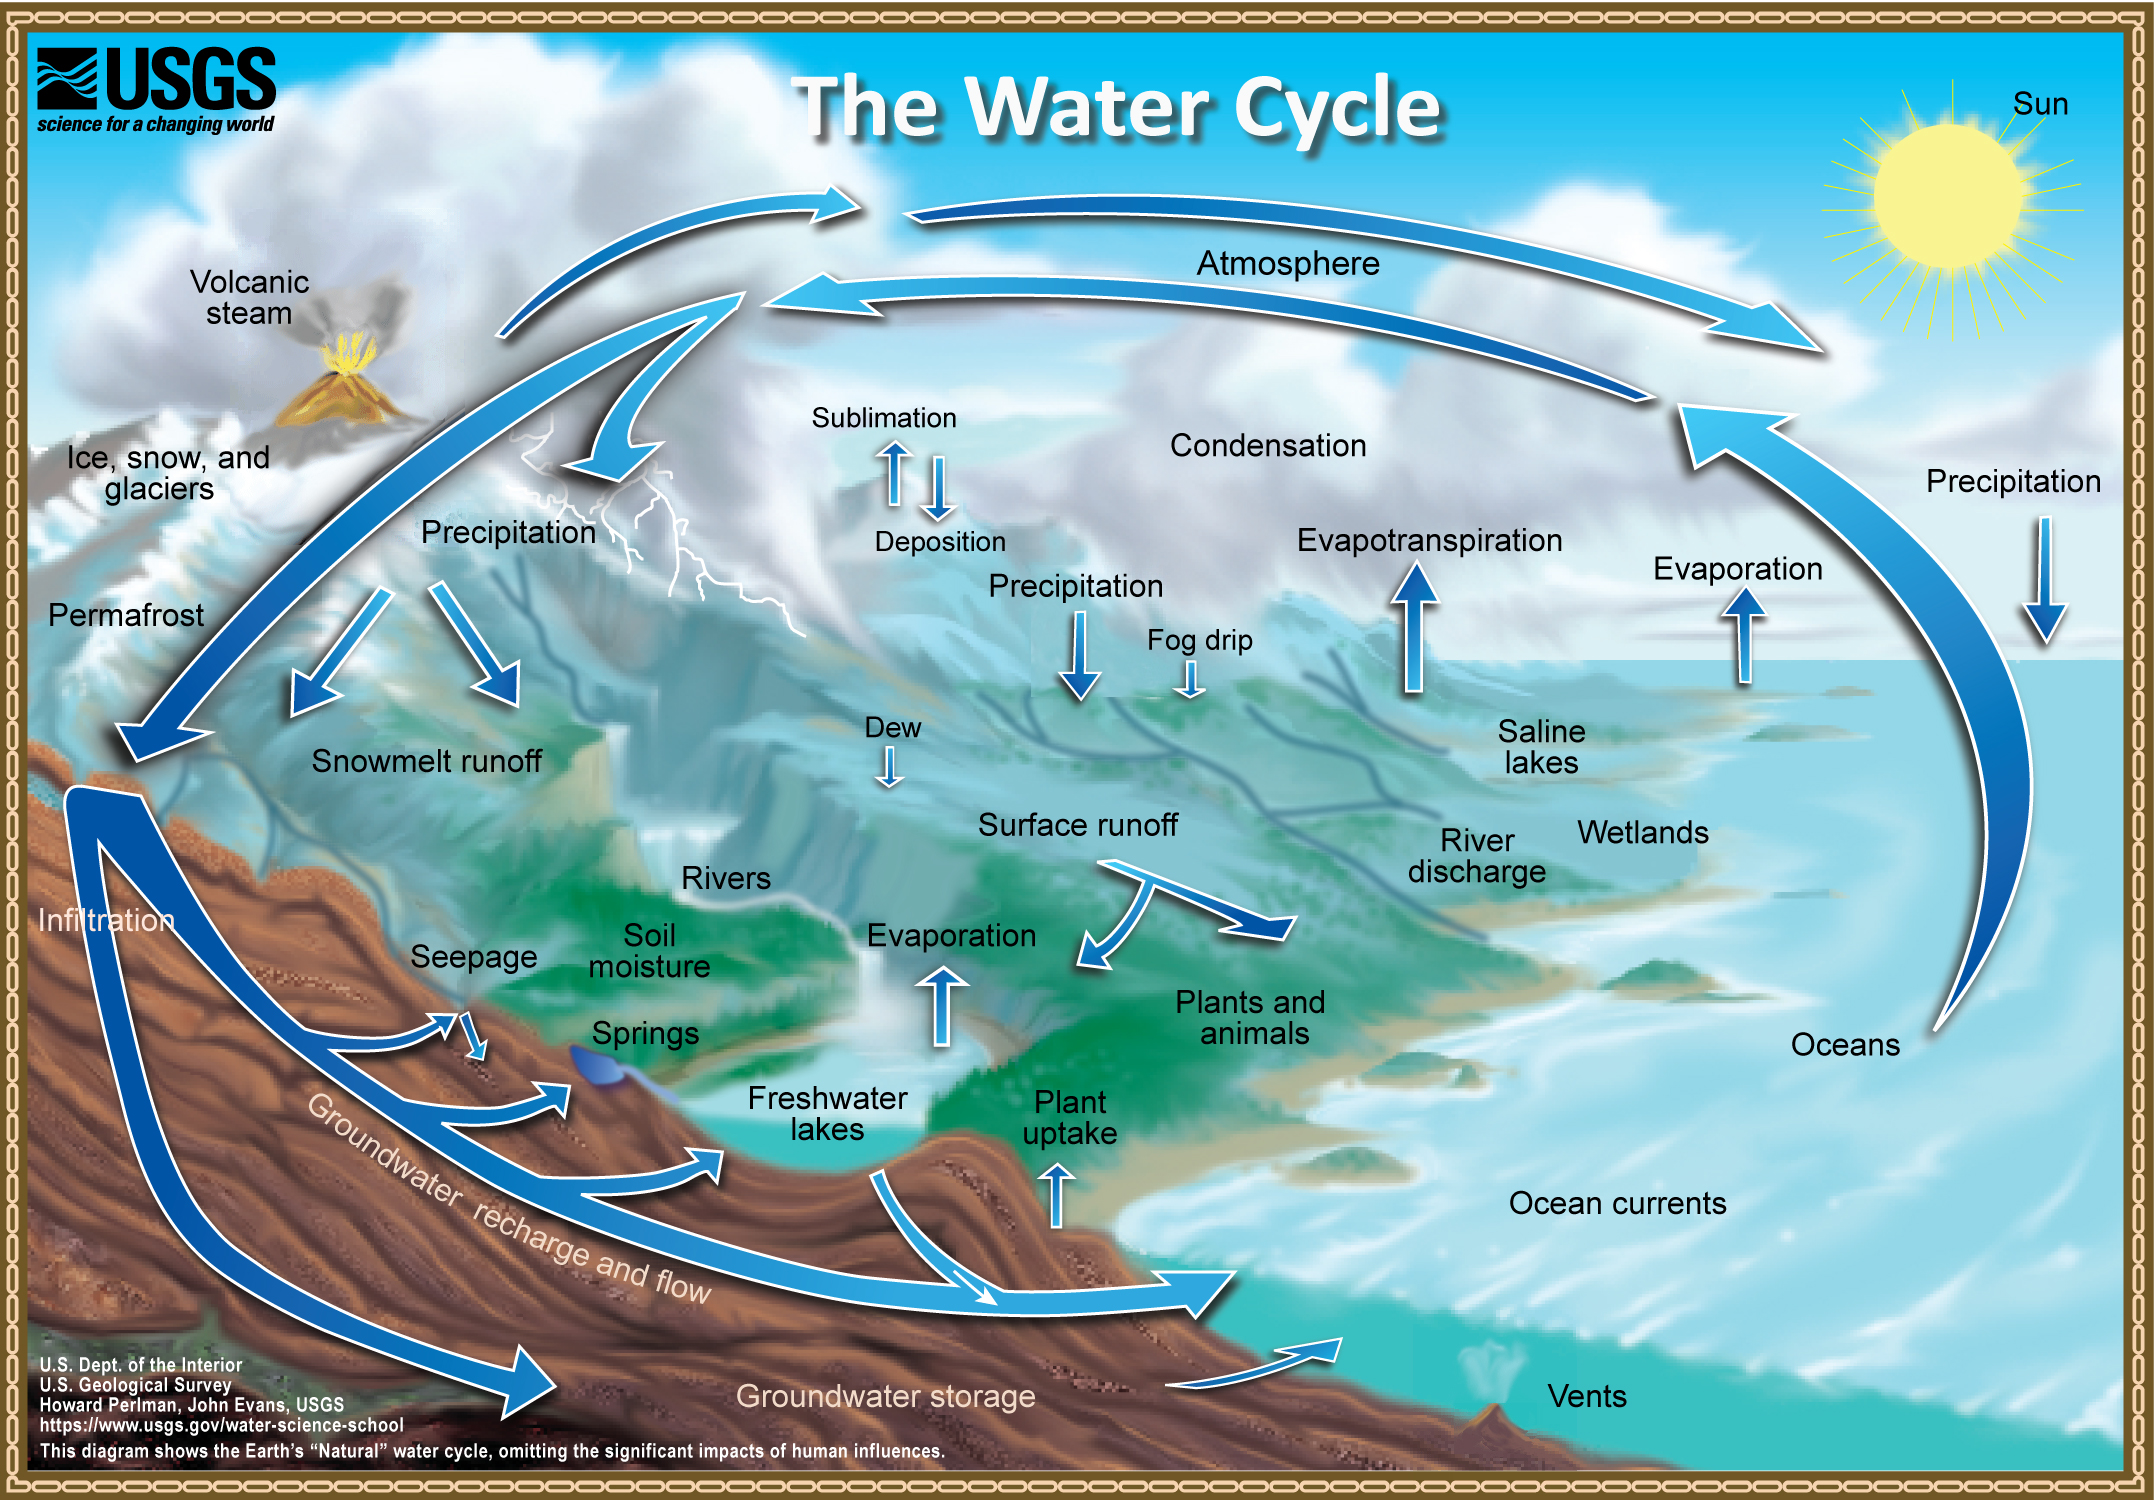
\includegraphics[width=0.7\textwidth]{water-cycle-natural} % Datei in "bilder/" bei LaTeX: eps, bei PDFLaTeX: jpg (o.ä.) 
	\caption{Horologic Cycle} 
	\label{fig:hydrologic cycle}
\end{figure}
\section{Observation from Satellite}
It was extremely difficult to measure the global water storage change consistently. In some way, remote sensing with satellite is the perfect tool for hydrology research, which has the ability to provide the data globally in a long term.\\\\
The GRACE twin satellites, launched 17 March 2002, are making detailed measurements of Earth's gravity field, which are caused by monthly changes in mass. The mass changes can be thought of as concentrated in a very thin layer of water thickness changes near the Earth's surface by moving ocean, atmospheric and land ice masses and by mass exchanges between these Earth system compartments. \\\\
There are 2 satellites with tandem polar orbit. Since the orbit is around the pole and the earth rotates itself, the satellites were able to get the whole view of the earth. Unlike the normal remote sensors, the GRACE satellites measured the gravity field of the earth. When the 2 satellites went over a mass anomaly like a big mountain, the distance of them will be a little bit smaller. By calculating this distance difference with the help of GPS system, the gravity field anomaly of the earth along with the total water storage anomaly are able to be plotted monthly. \\\\
It is shown, that GRACE delivers the highest temporal resolution and is thus able to observe monthly mass variation with a spatial resolution of less than 1000\ut{km}. In (Wahr et al., 1998) it was predicted that GRACE would be able to measure these effects with an accuracy of about 2\ut{mm} of water equivalent heights. Though this accuracy has not yet been achieved because of the errors in spherical harmonic coefficients of short-wavelength, it was shown in many publications that the Stokes coefficients from GRACE indeed contain hydrological signals as the monthly solutions from GRACE showed a good agreement with mass variations from hydrological models.
\begin{figure}[htbp]
	\centering
	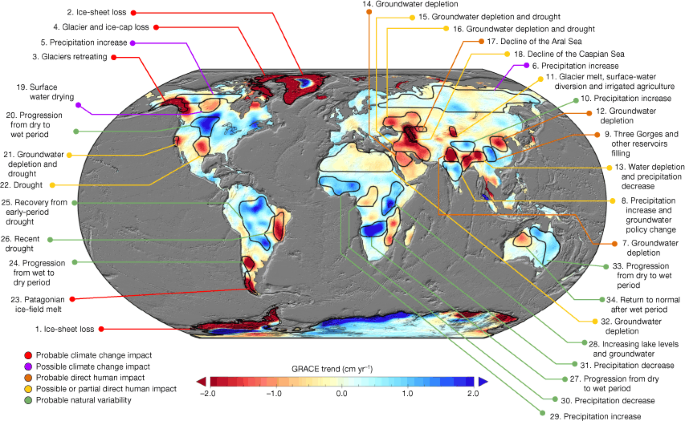
\includegraphics[width=0.6\textwidth]{TWSA} % Datei in "bilder/" bei LaTeX: eps, bei PDFLaTeX: jpg (o.ä.) 
	\caption{Water Storage Change} 
	\label{fig:TWSA}
\end{figure}
\begin{figure}[ht]
	\centering
	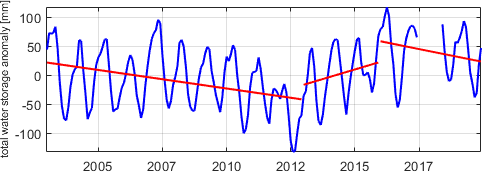
\includegraphics[width=0.6\textwidth]{Obbasin} % Datei in "bilder/" bei LaTeX: eps, bei PDFLaTeX: jpg (o.ä.) 
	\caption{Ob basin} 
	\label{fig:Obbasin}
\end{figure}\\
\section{Motivation}
A time series is a series of data points indexed (or listed or graphed) in time order. Most commonly, a time series is a sequence taken at successive equally spaced points in time. Thus it is a sequence of discrete-time data.  In hydrology, most variables are observed in time series, including Total Water Storage Anomaly(TWSA). In the hydrological cycle, this should reflect seasonal behavior and is in long term relatively stable. However, it was shown that since 2002 the TWSA of many big basins has increased (see figure \ref{fig:TWSA}). One important basin of them is Ob basin in west Siberia (see figure \ref{fig:Obbasin}). How did this trend happen is a very interesting topic. Through the analysis of the trend of the time series, it is possible to further understand the changes that have taken place before and future changes can also be predicted based on the stationary analysis.
\section{Objective}
In this thesis, the beginning point of the changing trend is to be found by analyzing the TWSA time series from GRACE data. In order to find the reason of the change, the precipitation, the evatranspiration along with the runoff in the same period from different data center would also be processed and compared with the TWSA. At the end, how was the changes of the TWSA and the reasons for this change would be discussed. 

\chapter{Study Area}
Ob River (\autoref{fig:Ob Basin}), river of central Russia. One of the greatest rivers of Asia, the Ob flows north and west across western Siberia in a twisting diagonal from its sources in the Altai Mountains to its outlet through the Gulf of Ob into the Kara Sea of the Arctic Ocean. It is a major transportation artery, crossing territory at the heart of Russia that is extraordinarily varied in its physical environment and population. Even allowing for the barrenness of much of the region surrounding the lower course of the river and the ice-clogged waters into which it discharges, the Ob drains a region of great economic potential.\\\\
\begin{figure}[htbp]
	\centering
	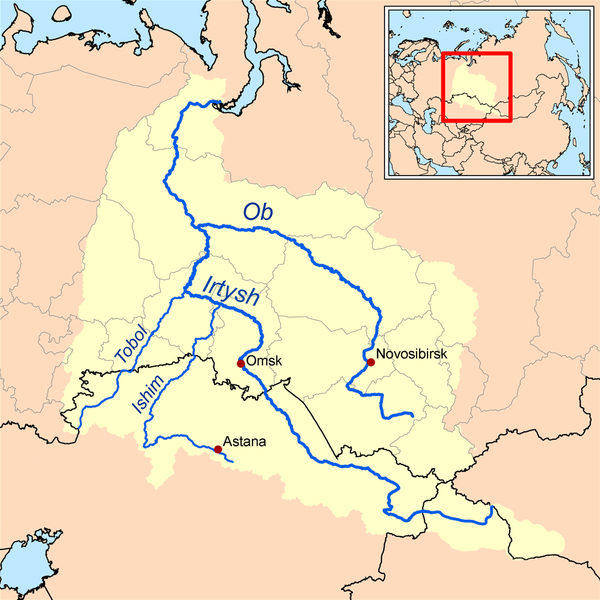
\includegraphics[width=0.7\textwidth]{Obbasin_area} % Datei in "bilder/" bei LaTeX: eps, bei PDFLaTeX: jpg (o.ä.) 
	\caption{River Basins Ob http://www.geologypage.com/2014/03/ob-river.html} 
	\label{fig:Ob Basin}
\end{figure}
\section{Physiography}
The Ob proper is formed by the junction of the Biya and Katun rivers, in the foothills of the Siberian sector of the Altai, from which it has a course of 3 650 km. If, however, the Irtysh River is regarded as part of the main course rather than as the Ob's major tributary, the maximum length, from the source of the Black (Chorny) Irtysh in China's sector of the Altai, is 5 410 km, making the Ob the seventh longest river in the world. The catchment area is approximately 2 975 000 square km. Constituting about half of the drainage basin of the Kara Sea, the Ob's catchment area is the sixth largest in the world. The drainage basin is classified as cropland (36\%), forest (30\%), wetland (11\%), grassland (10\%), shrub (5\%) , developed (5\%) and irrigated cropland (3\%).\cite{revenga1998watersheds}\\\\
The West Siberian Plain covers about 85 percent of the Ob basin.\cite{Obriver} The rest of the basin comprises the terraced plains of Turgay (Kazakhstan) and the small hills of northernmost Kazakhstan in the south and the Kuznetsk Alatau range, the Salair Ridge, the Altai Mountains and their foothills and outliers in the southeast.\\\\
The huge basin of the Ob stretches across a number of natural zones. Semidesert prevails in the far south around Lake Zaysan (recipient of the Black Irtysh and source of the Irtysh proper), bordered on the north by steppe grassland. The central regions of the West Siberian Plain i.e., more than half of the basin-consist of taiga (swampy coniferous forest), with great expanses of marshland. In the north there are vast stretches of tundra (low-lying, cold-tolerant vegetation).
\section{Climate}
\begin{figure}[htbp]
	\centering
	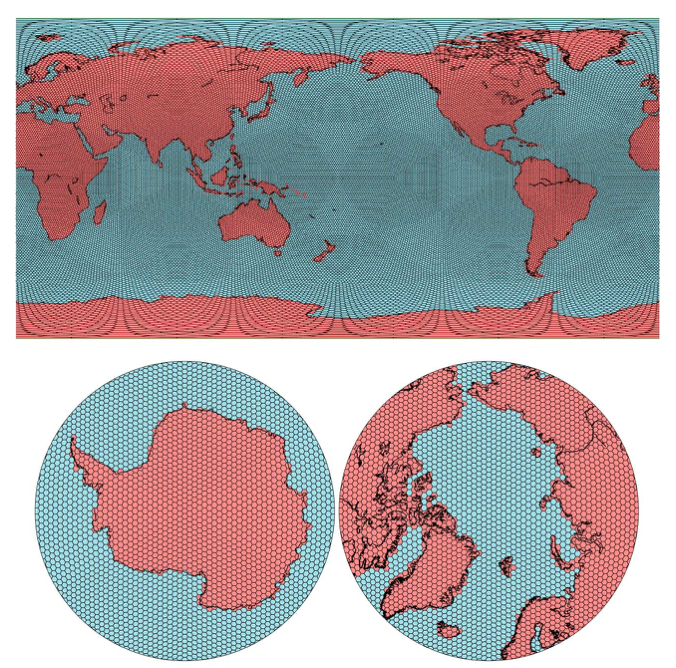
\includegraphics[width=0.5\textwidth]{mascon} % Datei in "bilder/" bei LaTeX: eps, bei PDFLaTeX: jpg (o.ä.) 
	\caption{The distribution of 40,962 geodesic grid tiles over the Earth used as a basis function for estimation of mass
		anomalies from GRACE for CSR mascon solutions. (top) Global view, (bottom left) South Pole view, and (bottom right) North Pole view \cite{save2016high}} 
	\label{fig:mascon}
\end{figure}
The Ob basin has short, warm summers and long, cold winters. Average January temperatures range from  $-28 ^{\circ}$C on the shores of the Kara Sea to $-16 ^{\circ}$C in the upper reaches of the Irtysh. July temperatures for the same locations, respectively, range from 4 $^{\circ}$C to above $20 ^{\circ}$C. The absolute maximum temperature, in the arid south, is $40 ^{\circ}$C,\cite{Obriver} and the minimum, in the Altai Mountains, is $-60 ^{\circ}$. Rainfall, which occurs mainly in the summer, averages less than 400 mm per year in the north, 500 to 600 mm in the taiga zone, and 300 to 400 mm on the steppes. The western slopes of the Altai receive as much as 1 575 mm per year. Snow cover lasts for 240 to 270 days in the north and for 160 to 170 days in the south. It is deepest in the forest zone, where it ranges from 60 to 90 cm, and in the mountains, where it averages 200 cm per year. It is much shallower on the tundra, ranging from 30 to 50 cm, and very thin on the steppe, where 20 to 40 cm fall.\cite{Obriver}\\\\
On the upper Ob the spring floods begin early in April, when the snow on the plains is melting; and they have a second phase, ensuing from the melting of snow on the Altai Mountains. The middle Ob, scarcely affected by the upper Ob's phases, has one continuous spring-summer period of high water, which begins in mid April. For the lower Ob, high water begins in late April or early May. Levels, in fact, begin to rise when the watercourse is still obstructed by ice; and maximum levels, which occur by May on the upper Ob, may not be reached until June, July, or even August on the lower reaches. For the upper Ob, the spring floods end by July, but autumn rains bring high water again in September and October; in the middle and lower Ob, the spring and summer floodwaters gradually recede until freezing sets in. On the lower reaches, flooding may last four months. Flooding of the Ob proper and of the Irtysh obstructs the minor tributaries' drainage.
\section{Hydrology}
The Ob has the third greatest discharge of Siberia's rivers, after the Yenisey and the Lena. On average, it pours some 400 cubic km of water annually into the Arctic Ocean about 12\% of that ocean's total intake from drainage.\\\\
The volume of flow at Salekhard, just above the delta, is about 42 000 cubic metres per second at its maximum and 2 000 cubic metres per second at its minimum, while for Barnaul, on the upper Ob, the corresponding figures are 9 600 and 200 cubic metres per second. The average annual discharge rate at the river's mouth is about 12 700 cubic metres per second. Most of the water comes from the melting of seasonal snow and from rainfall; much less of it comes from groundwater, mountain snow, and glaciers.\cite{Obriver}
\section{Plants and animals}
Pine, cedar, silver fir, aspen, and birch grow on the banks and occasionally constitute isolated forests on the higher ground of the floodplain. Large areas near the river are covered with willow, snowball trees, bird cherry, buckthorn, currant bushes, and wild roses.\\\\
Fur-bearing mammals of the Ob valley include European and Siberian mole, Siberian and American mink, ermine, fox, wolf (in the taiga), elk, white hare, water rat, muskrat, otter, and beaver. Among more than 170 species of birds breeding in the floodplain are grouse, partridge, goose, and duck.
\section{Human use}
Basin total population is about 27 million, with 39 cities having a population of more than 100 000. The Ob's immense hydroelectric potential is estimated at some 250 billion kilowatts. Three main stations have been built: one on the Ob proper, at Novosibirsk, and the other two on the mountainous reaches of the Irtysh, at Bukhtarma and Oeskemen. Both industry and agriculture have been intensively developed in the Ob basin. Cities such as Omsk, Novosibirsk, and Barnaul are major industrial and manufacturing centres. The steppe zone, in the southern Ob basin, is the major producer of spring wheat in Russia. The west Siberian oil and gas fields, located in the taiga and tundra zones of the middle and lower Ob, are the most important in Russia, contributing about two-thirds of the country's crude oil and natural gas output.

\ifiscorrect\linespread{1.0}\selectfont% Zeilenabstand wieder auf 1 zur�ck
\else\fi

% Setze Numerierung wieder auf r�misch zur�ck und setzte von oben fort
% Wert ist demnach der von 'roemisch'
\newpage
\pagenumbering{Roman}
\setcounter{page}{\value{roemisch}}

%% Literaturverzeichnis
\bibliography{literatur/bib}


%% Appendix, falls vorhanden
\appendix
\chapter{Estimating TWS from GRACE SH}\label{shmethod}
The shape of the geoid, i.e. the distance between the reference ellipsoid and the geoid surface $N$, can be expanded in a sum of spherical harmonics.
\begin{equation}
N(\theta, \lambda) = R \sum_{l=0}^{\infty} \sum_{m=0}^{l} \tilde{P}_{lm}(\cos \theta)(\tilde{C}_{lm} \cos m\lambda + \tilde{S}_{lm}\sin m\lambda)
\end{equation}
where
\begin{table}[htbp]
	\begin{tabular}{ll}	
		$N(\theta, \lambda)$	&  geoid height at a point with the spherical coordinates $\theta$,$\lambda$\\ 
		$R$	&  radius of the Earth\\ 
		$\tilde{P}_{lm}$	&  normalized associated Legendre functions of degree $l$ and order $m$\\ 
		$\tilde{C}_{lm}$,$\tilde{S}_{lm}$	&  normalized Stokes coefficients\\ 
	\end{tabular}
\end{table}
The time-dependent change in the geoid heights $\Delta N$ is reflected by the difference between the spherical harmonic coefficients $\tilde{C}_{lm}$,$\tilde{S}_{lm}$. In this case, the equation can be written as:
\begin{equation}
\Delta N(\theta, \lambda) = R \sum_{l=0}^{\infty} \sum_{m=0}^{l} \tilde{P}_{lm}(\cos \theta)(\Delta \tilde{C}_{lm} \cos m\lambda + \Delta \tilde{S}_{lm}\sin m\lambda)
\end{equation}
By assuming that $\Delta N(\theta, \lambda;t) \neq 0$, it is clear that there had to be a change in the Earth's gravity field caused by mass fluctuations in, on and above the Earth's surface. This change is denoted as a change in the Earth's density distribution. In\cite{wahr1998time}, it was found that there is a connection between this quantity and its representation in spherical harmonic coefficients.
\begin{equation}
\begin{Bmatrix}
\Delta \tilde{C}_{lm}(t)\\
\Delta \tilde{S}_{lm}(t)
\end{Bmatrix} = \frac{3}{4\pi R \rho_{ave}(2l+1)} \int \int \Delta \rho(r,\theta,\lambda;t) \tilde{P}_{lm}(\cos \theta) \times (\frac{r}{R})^{l+2} \begin{Bmatrix}
\cos m\lambda \\
\sin m\lambda
\end{Bmatrix} \sin\theta d\theta d\lambda
\end{equation}
where $r$ is the distance of the computation point from the center of the Earth and $\rho_{ave}$ is the average density of the Earth. However, an accurate determination of $\Delta \rho(r,\theta,\lambda;t)$ is nearly impossible, because it requires prior knowledge about the inner density distribution of the Earth. But all short periodic mass variations can be assumed to happen only in a thin layer on the Earth's surface, which can be detected by GRACE satellites. The thickness is mostly determined by the thickness of the atmosphere and is of the order of 10 to 15 \ut{km} \cite{wahr1998time}. \\\\
The change in this thick layer is called surface density $\Delta \rho_{S}$, which can be defined as the radial integral of $\Delta \rho$ through this layer and since the layer is thick enough, it can be assumed that $r \approx R$, so the equation can be simplified as
\begin{equation}
\begin{Bmatrix}
\Delta \tilde{C}_{lm}(t)\\
\Delta \tilde{S}_{lm}(t)
\end{Bmatrix}_{\text{surf mass}} = \frac{3}{4\pi R \rho_{ave}(2l+1)} \int \int \Delta \rho(\theta,\lambda;t) \tilde{P}_{lm}(\cos \theta)  
\begin{Bmatrix}
\cos m\lambda \\
\sin m\lambda
\end{Bmatrix} \sin\theta d\theta d\lambda
\end{equation}
This equation now connects the density redistribution in this thin layer with the spherical harmonic coefficients. Thus, it describes the contribution to the geoid from the direct gravitational attraction of the surface mass \cite{wahr1998time}. The mass fluctuations on the surface also deform the underlying Earth, which implicates a change in the gravitational potential, and thus a change in the geoid shape, as well. This effect is considered by the so called $Love\ number\ k_{l}$, which were derived from\cite{han1995viscoelastic}. The contribution from the deformed solid earth may then be written as
\begin{equation}
\begin{Bmatrix}
\Delta \tilde{C}_{lm}(t)\\
\Delta \tilde{S}_{lm}(t)
\end{Bmatrix}_{\text{solid Earth}} = \frac{3k_{l}}{4\pi R \rho_{ave}(2l+1)} \int \int \Delta \rho(\theta,\lambda;t) \tilde{P}_{lm}(\cos \theta) 
\begin{Bmatrix}
\cos m\lambda \\
\sin m\lambda
\end{Bmatrix} \sin\theta d\theta d\lambda
\end{equation}
The total geoid change is obtained by adding (3.4) and (3.5)
\begin{equation}
\begin{Bmatrix}
\Delta \tilde{C}_{lm}(t)\\
\Delta \tilde{S}_{lm}(t)
\end{Bmatrix} = \begin{Bmatrix}
\Delta \tilde{C}_{lm}(t)\\
\Delta \tilde{S}_{lm}(t)
\end{Bmatrix}_{\text{surf Earth}} + \begin{Bmatrix}
\Delta \tilde{C}_{lm}(t)\\
\Delta \tilde{S}_{lm}(t)
\end{Bmatrix}_{\text{solid Earth}}
\end{equation}
Inserting (3.6) into (3.2) leads to the so called \textit{isotropic transfer coefficients}, which define the quantity of a spherical harmonic series expansion. In the case of a surface mass density, they are defined as 
\begin{equation}
\Lambda_{l} = \frac{R\rho_{ave}}{3} \frac{2l+1}{1+k_{l}}
\end{equation} 
Then an expression for the surface mass density in terms of the spherical harmonic coefficients can be written as
\begin{equation}
\Delta \rho_{S}(\theta,\lambda) = \frac{R \rho_{ave}}{3} \sum_{l=0}^{\infty} \frac{2l+1}{1+k_{l}} \sum_{m=0}^{l} \tilde{P}_{lm} (\cos \theta) (\Delta \tilde{C} \cos m \lambda + \Delta \tilde{S} \sin m \lambda)
\end{equation}
The gravity field change can be assumed as the change of the thin layer of water on the Earth's surface. The relation between the water equivalent heights and the surface mass density is
\begin{equation}
h_{W}(\theta,\lambda) = \frac{\Delta \rho_{S}(\theta,\lambda)}{\rho_{W}}
\end{equation}
where $\rho_{W}$ is the average density of water and thus
\begin{equation}
h_{W}(\theta,\lambda;t) = \frac{R \rho_{ave}}{3\rho_{W}} \sum_{l=0}^{\infty} \frac{2l+1}{1+k_{l}} \sum_{m=0}^{l} \tilde{P}_{lm} (\cos \theta) (\Delta \tilde{C} \cos m \lambda + \Delta \tilde{S} \sin m \lambda)
\end{equation}
For simplicity, this formula can be written as 
\begin{equation}
h_{W}(\theta,\lambda;t) = \sum_{l=0}^{\infty} \Lambda_{l} \sum_{m=0}^{l} \tilde{Y}_{lm}(\theta,\lambda) \Delta \tilde{K}_{lm}(t)
\end{equation}
where 
\begin{itemize}
	\item $\Lambda_{l} = \frac{R \rho_{ave}}{3 \rho w} \frac{2l+1}{1+k_{l}}$: isotropic spectral transfer coefficients
	\item $\tilde{Y}_{lm}(\theta,\lambda) = \tilde{P}_{lm}(\cos \theta)(\cos m\lambda \quad \sin m \lambda)^{T}$: normalized surface spherical harmonics
	\item $ \Delta \tilde{K}_{lm}(t) = (\Delta \tilde{C}_{lm} \quad \Delta \tilde{S}_{lm})^{T}$: normalized Stokes coefficients
\end{itemize}
The associated Legendre functions are given by
\begin{equation}
\tilde{P}_{n,m}(t) = \sqrt{(2-\delta_{m0})(2n+1)\frac{(n-m)!}{(n+m)!}}\sqrt{1-t^2}^{m}\frac{d^{n+m}}{dt^{n+m}}\frac{1}{2^n n!}(t^2 - 1)^n
\end{equation}
where $n$ is degree, $m$ is order and $t= \cos \theta$ is a substitution. The Legendre functions can be calculated by the recursion.
\begin{gather}
\tilde{P}_{0,0}(t) = 1 \\
\tilde{P}_{m,m}(t) = W_{m,m}\sin \theta \tilde{P}_{m-1,n-1}(t-1) \quad  \text{for $m > 0$ and $m =n$} \\
\tilde{P}_{n,m} = W_{n,m}[\cos \theta \tilde{P}_{n-1,m}(t) - \frac{1}{W_{n-1,m}} \tilde{P}_{n-2,m}(t)] \quad \text{for $m \neq n$}
\end{gather}       
with the factors
\begin{equation}
W_{n,m} = \begin{cases}
\sqrt{3} & \text{for $n = 1$ and $m = {0,1}$}\\
\sqrt{\frac{2n+1}{2n}} & \text{if $n=m$ and $n>1$} \\
\sqrt{\frac{(2n+1)(2n-1)}{(n+m)(n-m)}} & \text{$n>1$ and $m \neq n$}
\end{cases}
\end{equation}                   
and the convention $\tilde{P}_{n,m}(t) = 0$ for  $m>n$. This algorithm is shown to be stable until degree $n \approx 1800$. In this thesis they are up to 96. \\\\
It is obvious that only $\Delta \tilde{K}_{lm}$ is time dependent while $\Lambda_{l}$ and $\tilde{Y}_{lm}(\theta,\lambda)$ are constant in time, by using the methods of forwards and backward-differences a rate of mass variations in terms of water equivalent heights can be obtained.
\begin{equation}
\dot{h}_{W}(\theta,\lambda;t) = \sum_{l=0}^{\infty} \Lambda_{l} \sum_{m=0}^{l} \tilde{Y}_{lm}(\theta,\lambda) \Delta \dot{\tilde{K}}_{lm}(t)
\end{equation}
This computation of the area weighted rate of change of water equivalent heights ofr one particular region $\chi$, defined by a set of $k$ grid cell centers $(\theta_{i}, \lambda_{i}),j=1,2,3\cdots,k$, can be done according to
\begin{equation}
\dot{h}_{W}(\chi;t) = \sum_{j=1}^{k}\ \frac{a(\theta_{i},\lambda_{i})}{a(\chi)} sum_{l=0}^{\infty} \Lambda_{l} \sum_{m=0}^{l} \tilde{Y}_{lm}(\theta_{i},\lambda_{i}) \Delta \dot{\tilde{K}}_{lm}(t)
\end{equation}
\begin{table}[htbp]
	\begin{tabular}{ll}
		$\dot{h}_{W}(\chi;t)$	&  rate of mass change in catchment $\chi$\\ 
		$k$	&  number of date points in the catchment\\ 
		$a(\theta_{i},\lambda_{i})$	&  area of the grid cell $j$\\ 
		$a(\chi)$	&  total area of the catchment $\chi$\\ 
	\end{tabular}
\end{table}
In this thesis, the size of the cell is $0.5^{\circ} \times 0.5^{\circ}$, which means there are $360 \times 720$ cells.
With the help of the \textit{shbundle}, \textit{EWHbundle} and the basin mask from the Institute of Geodesy (GIS), University of Stuttgart, this process can easily be done and the equivalent water heights of Ob area between 2002 and 2020 are acquirable. 

\end{document}
